\chapter{Signal Processing}
\begin{itemize}
\item[white noise]White noise is the noise signal whose power spectrum is flat i.e. will have almost constant integrated power at different frequency bands of same duration (bandwidth). White noise is made of almost all the frequencies and will have constant power at all these frequencies; hence it is also analogous to white light emitting all the frequencies in the same proportion. The figure describes spectrum of white noise.
\begin{figure}[h!]
  \centering
  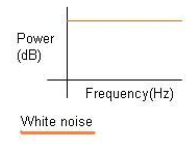
\includegraphics[scale=0.45]{images/I/wn.png}
  \caption{White noise}\label{fig:wn}
\end{figure}

\item[coloured noise]Colored noise will have different integrated power at different frequency bands of same duration. Depending upon whether it is gray, pink, blue or brown color it will have different power spectrum. Based on this power concentration varies at different frequencies. The figure describes spectrum of colored noise(example-Pink noise).
\begin{figure}[h!]
  \centering
  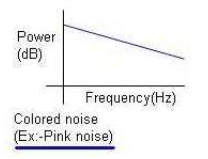
\includegraphics[scale=0.45]{images/I/cn.png}
  \caption{Coloured noise}\label{fig:cn}
\end{figure}


\item[Husid Plot] A plot of the build-up of Arias intensity with
time is known as a Husid plot (Figure 6) and it serves
to identify the interval over which the majority of
the energy is imparted. The root-mean-square acceleration (arms) is the equivalent constant level of
acceleration over any specified interval of the accelerogram; the arms is also the square root of the gradient of the Husid plot over the same interval. Arias
intensity has been found to be a useful parameter to
define thresholds of shaking that trigger landslides.
\begin{figure}[h!]
  \centering
  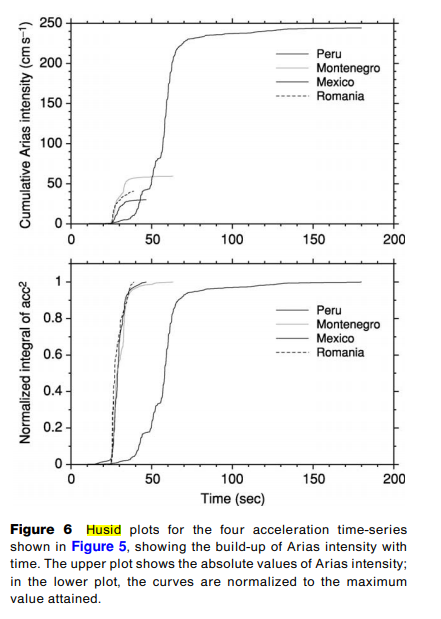
\includegraphics[scale=0.45]{images/I/husid.png}
  \caption{Husid Plot}\label{fig:husid}
\end{figure}
\end{itemize}


